\chapter{Probabilistic Inference for Error Detection in De Novo Genome Assemblies}
\label{chap:illumina}
\section{Overview}
This chapter presents results in a different research domain than the previous three chapters. Instead of confocal single-molecule  fluorescence, here we consider gene sequencing using Illumina's fluorescence-based sequencing technology~\cite{bentley2008}. We describe the development and evaluation of an error detection tool, NxRepair~\cite{murphy2015}, designed to locate and correct misassemblies in \textit{de novo} assemblies of bacterial genomes constructed using Illumina Nextera mate pair~\cite{nextera2012} sequencing. In a \textit{de novo} sequence assembly, scaffolding errors and incorrect repeat disambiguation during \textit{de novo} assembly can result in large scale misassemblies in draft genomes. Nextera mate pair sequencing data provide additional information to resolve assembly ambiguities and prevent these errors. However, despite this additional information, mistakes can still occur. We show, through comparison with matched refernence genomes, that the NxRepair tool can quantitatively improve the quality of \textit{de novo} assemblies and that it outperforms other error detection tools in identifying large-scale misassemblies. The work presented here was completed during an internship at Illumina Cambridge.

This chapter opens with a brief overview of sequencing technologies and their relationship to fluorescence microscopy. We then introduce the problem of \textit{de novo} genome assembly and discuss prior methods for error detection in genome assemblies. Following this introduction, we describe the development of our NxRepair tool, which uses a probabilistic analysis to identify regions of a \textit{de novo} assembly that have a high probability of containing an error. Finally, we evaluate the performance of NxRepair on a series of nine bacterial genomes. We show that NxRepair can identify and correct large scaffolding errors, without use of a reference sequence, resulting in quantitative improvements in the assembly quality. We close this chapter by discussing the potential applicatons of this tool, but also the limitations of this approach to error detection. NxRepair can be downloaded from GitHub; a tutorial and user documentation are also available.
 

\section{Introduction}
\subsection{Next-Generation Sequencing Technologies}
Sequencing is the determination of the sequence of base pairs in a strand of DNA. Since the completion of the first complete genome sequence~\cite{sanger1977}, there have been huge developments in the technology used both to read the seqeunce of DNA bases and to assemble those reads into a complete genome. The first genome sequencing experiments used polymerisation reactions with a reaction mixture containing both radiolabelled deoxynucleotidetriphosphates (dNTPs) and radiolabelled di-deoxynucleotidetriphosphates (ddNTPs), which terminate chain elongation at specific bases. The elongation reaction was carried out four times, each time using a different ddNTP, so that fragments in one reaction mixture would all terminate with the same base. Following elongation, the newly constructed framgments from the four reaction mixtures were run out on a high-resolution gel and the sequence read out manually based on the fragment position and the ddNTP used in the elongation reaction (Fig.~\ref{fig:sanger},~\cite{sanger1977}). However, this method of sequencing was laborious, slow and expensive, significantly limiting the widespread application of DNA sequencing technologies~\cite{metzker2005}. The development of fluorescent nucleotide labels~\cite{Smith1985}, initially enabling sequencing from a single elongation reaction (Fig.~\ref{fig:sanger}~\cite{Smith1986}) combined with methods for automating and paralellizing the sequencing reactions created the field of high-throughput, or next-generation, sequencing (NGS).


\begin{figure*}
\centerline{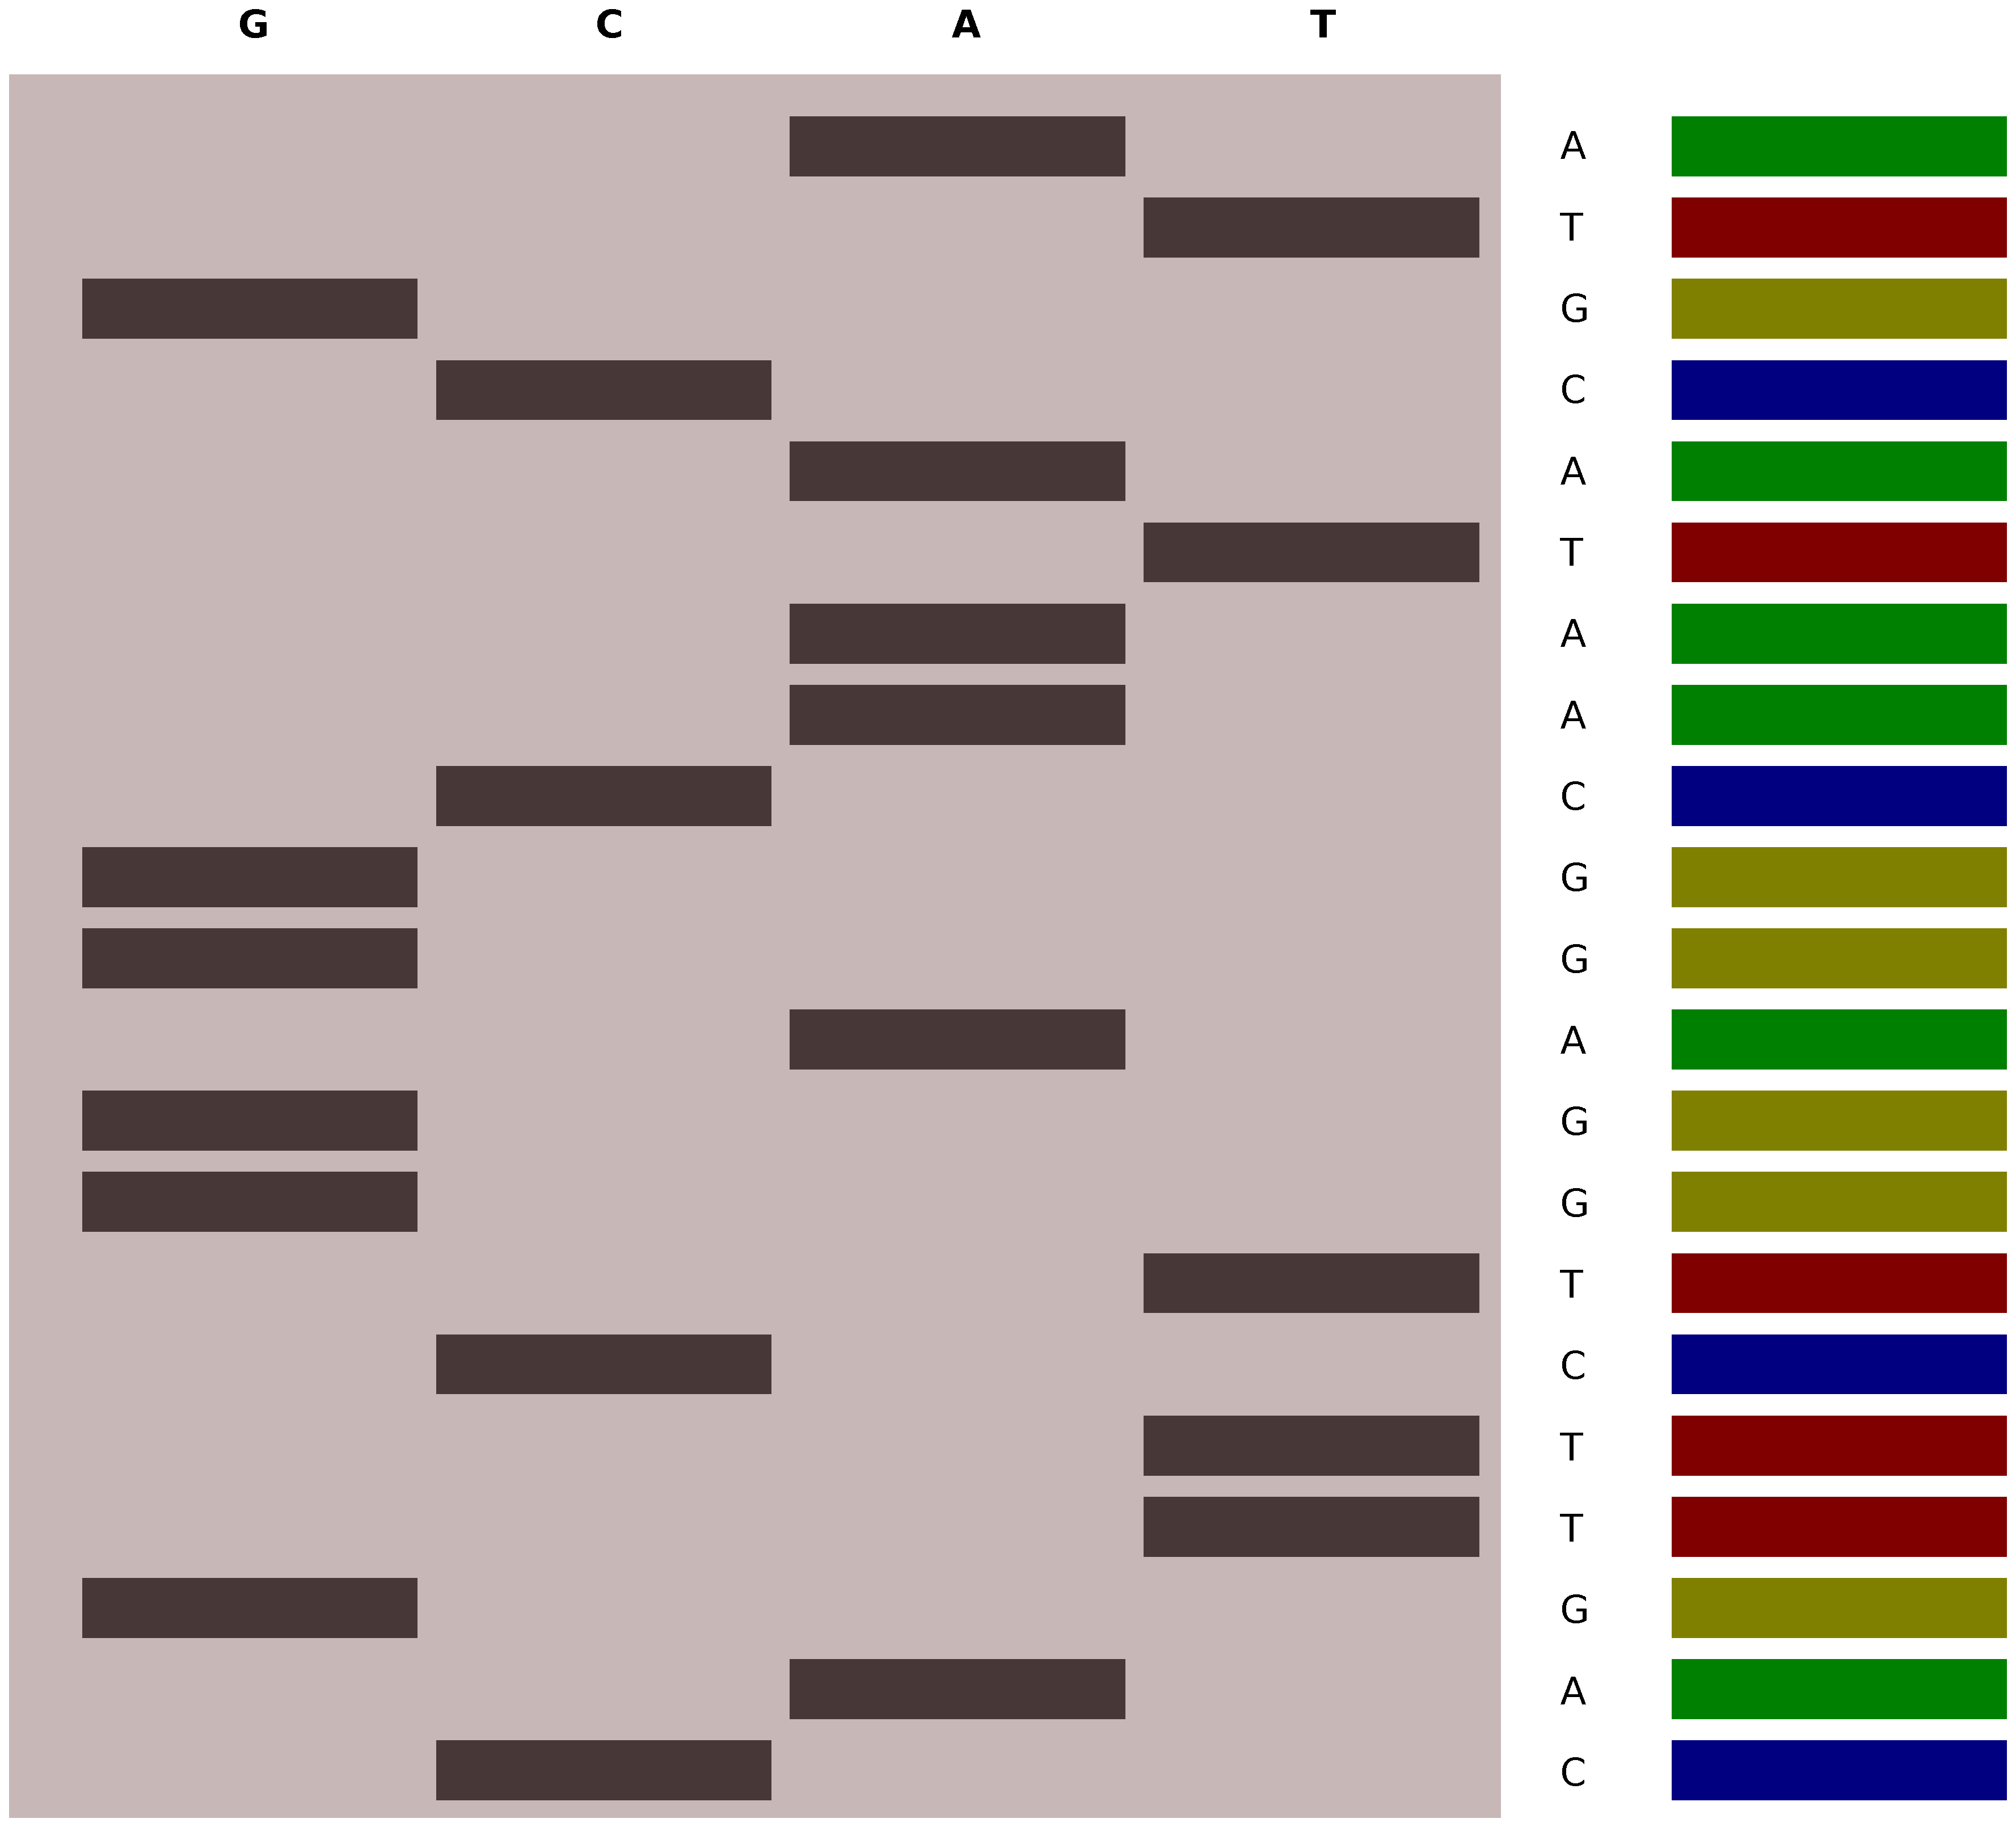
\includegraphics[width=0.8\textwidth]{illumina/sanger.pdf}}
\caption{Schematic of Sanger Sequencing using terminator chemistry. Left: sequencing on a four-lane gel. Four lanes represent sequencing mixtures containing different ddNTPs. Right: Sanger sequencing in a single lane using fluorescently labelled ddNTPs. Middle: the corresponding DNA sequence.}
\label{fig:sanger}
\end{figure*} 

\paragraph{Illumina Sequencing Technology}
The most popular, and best known, NGS technology is Illumina's sequencing by synthesis~\cite{illumina2010}. In the Illumina sequencing pipeline, DNA strands are fragmented into short pieces and attached to specific adapter sequences. The modified sequences are introduced to the Illumina flowcell, locally amplified in a ``clustering" reaction~\cite{Adessi2000} and then cycled through repeated elongation and imaging steps, to read out the DNA sequence one nucleotide at a time (Fig.~\ref{fig:illumina}). Illumina sequencing is a fluorescence-based technology. It uses reversible terminator chemistry to elongate a templated DNA molecule by a single base, using a dye-labelled nucleotide bearing a terminator group to prevent further elongation. The DNA base is identified based on the fluorescence emission of the attached dye. Following imaging, the terminator group and dye are removed and the next terminated nucleotide introduced at the now exposed hydroxyl group (Fig.~\ref{fig:terminator}). 

\begin{figure*}
\centerline{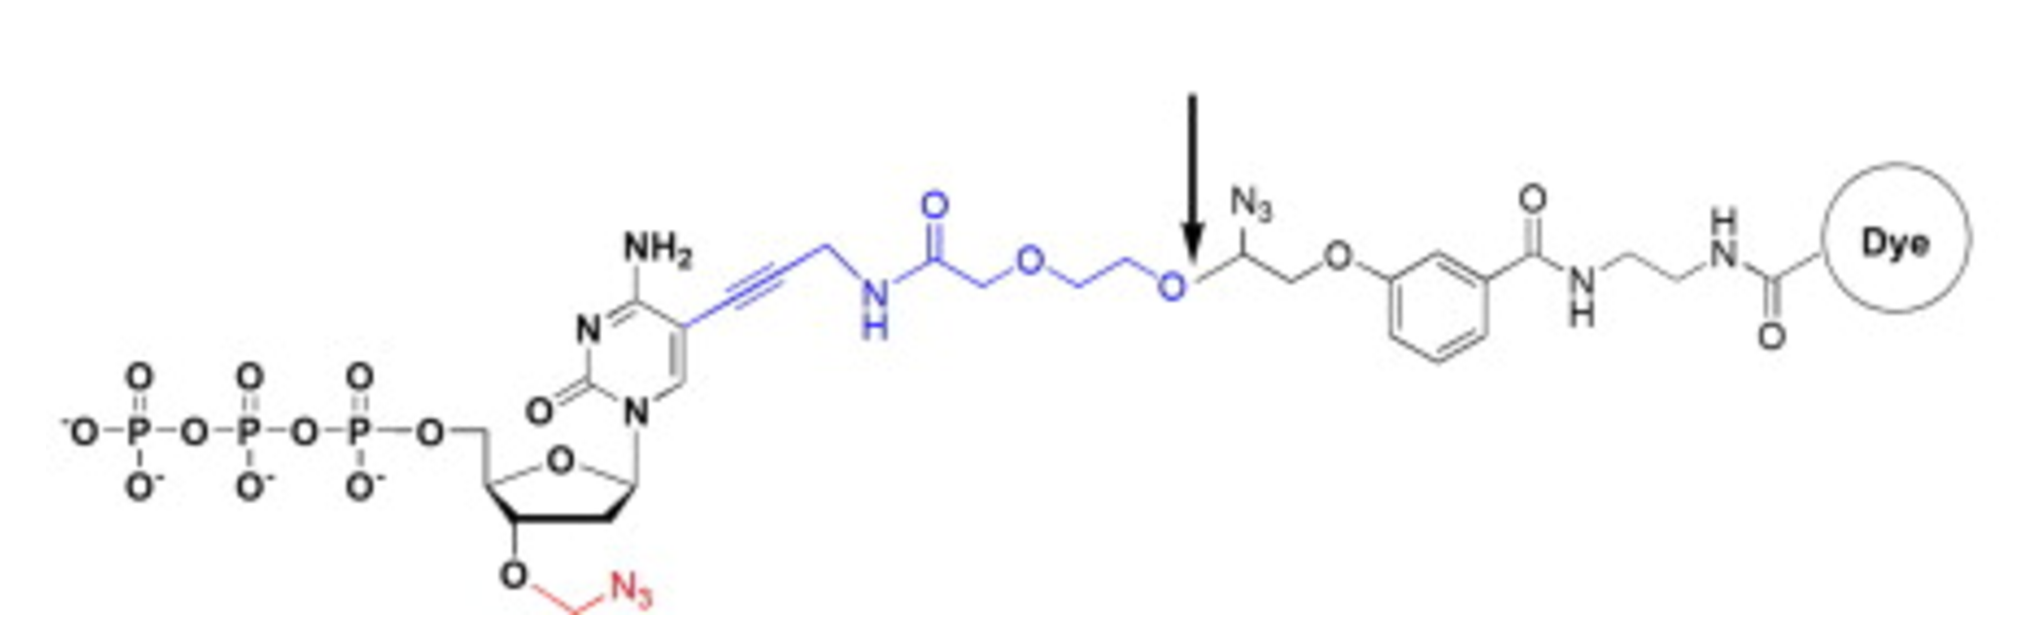
\includegraphics[width=0.8\textwidth]{illumina/illumina_linker.pdf}}
\caption{A modified nucleotide showing Illumina terminator chemistry. The 3'-hydroxyl group is reversibly blocked by the 3′-O-azidomethy terminator (red atoms), whilst the fluorescent indicator dye can be reversibly cleaved from the modified DNA base at the bond indicated by the arrow. Figure adapted from~\cite{Chen2013}}
\label{fig:terminator}
\end{figure*}  

Illumina's sequencing technology is a fluorescence based imaging technique. However, there are several major differences between this sequencing process and the single-molecule confocal experiments described in the previous chapters. Firstly, rather than freely diffusing molecules imaged by a laser beam, the fluorescently labelled sequences are tethered to the flow-cell base and imaged using multiple cameras and epifluorescent illumination (see Section~\ref{subsect:techniques}). Secondly, unlike in a smFRET experiment, the imaging step does not attempt to distinguish individual fluorophores against a noisy background signal. Instead, the clustering step prior to imaging produces multiple, spatially localised copies of the same DNA sequence, hugely amplifying the available fluorescent signal. 

\begin{figure*}
\centerline{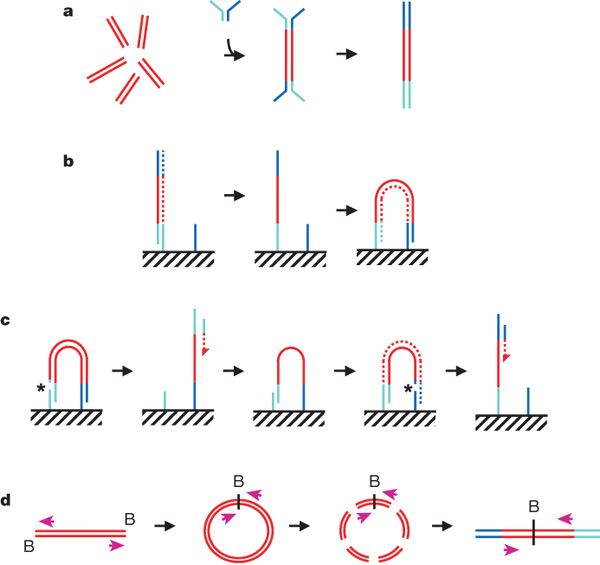
\includegraphics[width=0.8\textwidth]{illumina/illumina_sequencing.jpg}}
\caption{Sequencing by synthesis. A) DNA fragments are generated and joined to a pair of oligonucleotides. The ligated products are amplified using two oligonucleotide primers, resulting in double-stranded blunt-ended material with a different adaptor sequence on either end. B) DNA fragments are denatured and single strands are annealed to complementary oligonucleotides on the flow-cell surface. A new strand is copied from the original strand in an extension reaction; the original strand is then removed by denaturation. Multiple cycles of annealing, extension and denaturation in isothermal conditions result in cluster growth. C) The DNA in each cluster is linearized by cleavage within one adaptor sequence and denatured, generating single-stranded templates. D) Long-range paired-end sample preparation. The ends of each long fragment are tagged by incorporation of biotinylated (B) nucleotide and then circularized, forming a junction between the two ends. Circularized DNA is randomly fragmented and the biotinylated junction fragments are recovered and used as starting material in the standard sample preparation procedure. Figure and (adapted) caption from~\cite{bentley2008}.}
\label{fig:illumina}
\end{figure*} 

\paragraph{Single-Molecule Sequencing Technologies}
Although Illumina does not use single-molecule imaging, several other sequencing methods do sequence individual DNA molecules. Single-Molecule Real Time Sequencing (SMRT)~\cite{eid2008} is another fluorescence based sequencing technology. In SMRT, DNA polymerase molecules are immobilized within the detection region of a zero-mode waveguide (ZMW). Fluorescently labelled dNTPs are incorporated by the polymerase and imaged in real time. The ZMW, an aluminium-coated glass slide, containing multiple nano-scale pinhole apertures, creates a zeptolitre detection volume, enabling detection of the nucleotide currently under incorporation, despite a relatively high ($\mu$M) concentration of labelled oligonucleotides~\cite{Levene2003}. SMRT, used in Pacific Biosciences sequencing technologies, is currently extremely expensive, but produce sequences with an average read length of 3000 nucleotides~\cite{Roberts2013}, compared with the 151 or 251 bases typical of an Illumina read.

A second, currently experimental, single-molecule sequencing technique is under development by Oxford Nanopore~\cite{Bayley2014}. This sequencing method uses electrophoresis to drive long DNA molecules through a nano-scale pore. Application of a voltage across the nanopore causes a flow of ions through the pore, creating a measurable current. DNA is negatively charged, so can also be drawn through the pore, causing variations in the observed current that are dependent on the DNA bases currently occupying the pore~\cite{Branton2008}. In principle, this allows a direct read-out of the base sequence; in practice several challenges, including control of the speed of strand progression through the pore and achieving individual base resolution~\cite{Laszlo2014}, mean that although nanopore sequencing can produce very long reads (average 5000 bases), these have a high error rate including systematic errors~\cite{Mikheyev2014}.  

\subsection{De Novo Sequence Assembly}
As described above, Illumina NGS produces reads of length 151 or 251 bases. Even a small bacterial genome has a total genomic size of several million bases. Consequently, one of the most challenging aspects of genome sequencing is to piece together the short fragments of sequence obtained from the sequencer into one or more contiguous sequences, corresponding to correctly reconstructed sections of the genome. This process of attempting to generate a complete genome from short reads is termed \textit{de novo} sequence assembly; it is distinct from, for example, sequence alignent~\cite{Li2010}, in which short reads are aligned against a previously constructed reference genome for the same organism, allowing identification of polymorphisms and small differences from the reference genome. 

\textit{De novo} assembly is the construction of a long, contiguous genomic sequence from short DNA reads, without using a reference genome. The most popular method of \textit{de novo} assembly contstructs a de Bruijn overlap graph~\cite{Compeau2011} from even shorter fragments, termed $k$-mers, generated by fragmenting the short reads, then traverses this graph to reconstruct the genome sequence. De Bruijn graph traversal as a method of assembly was proposed as early as 2001~\cite{Pevzner2001}; however the method only gained popularity once the first de Bruijn assemblers were released~\cite{Zerbino2008}. In the simplest case, the graph is constructed from single end reads. However, with only single end reads, disambiguating repeat regions, which tangle the de Bruijn graph, remains challenging. 

In de Bruijn graph assembly, the sequencing reads are subdivided into all possible shorter reads of length $k$, termed $k$-mers. A $k$-mer is described as having a prefix (the first $k - 1$ nucleotides) and a suffix (the last $k - 1$ nucleotides). A graph is then constructed, in which observed prefixes and suffixes are represented as nodes; a directed edge is drawn between two nodes if the $k$-mer representing that prefix-suffix pair is present in the sequencing data (Fig.~\ref{fig:de-bruijn}). The challenge of constructing the \textit{de novo} assembly is then addressed by constructing a continuous path through the resulting de Bruijn graph, in which every edge is visited. Such a path is termed an Eulerian cycle; efficient algorithms exist to find such cycles and many have been implemented for the \textit{de novo} assembly application~\cite{Zerbino2008, Bankevich2012, Li2010_SOAP}. 

\begin{figure*}
\centerline{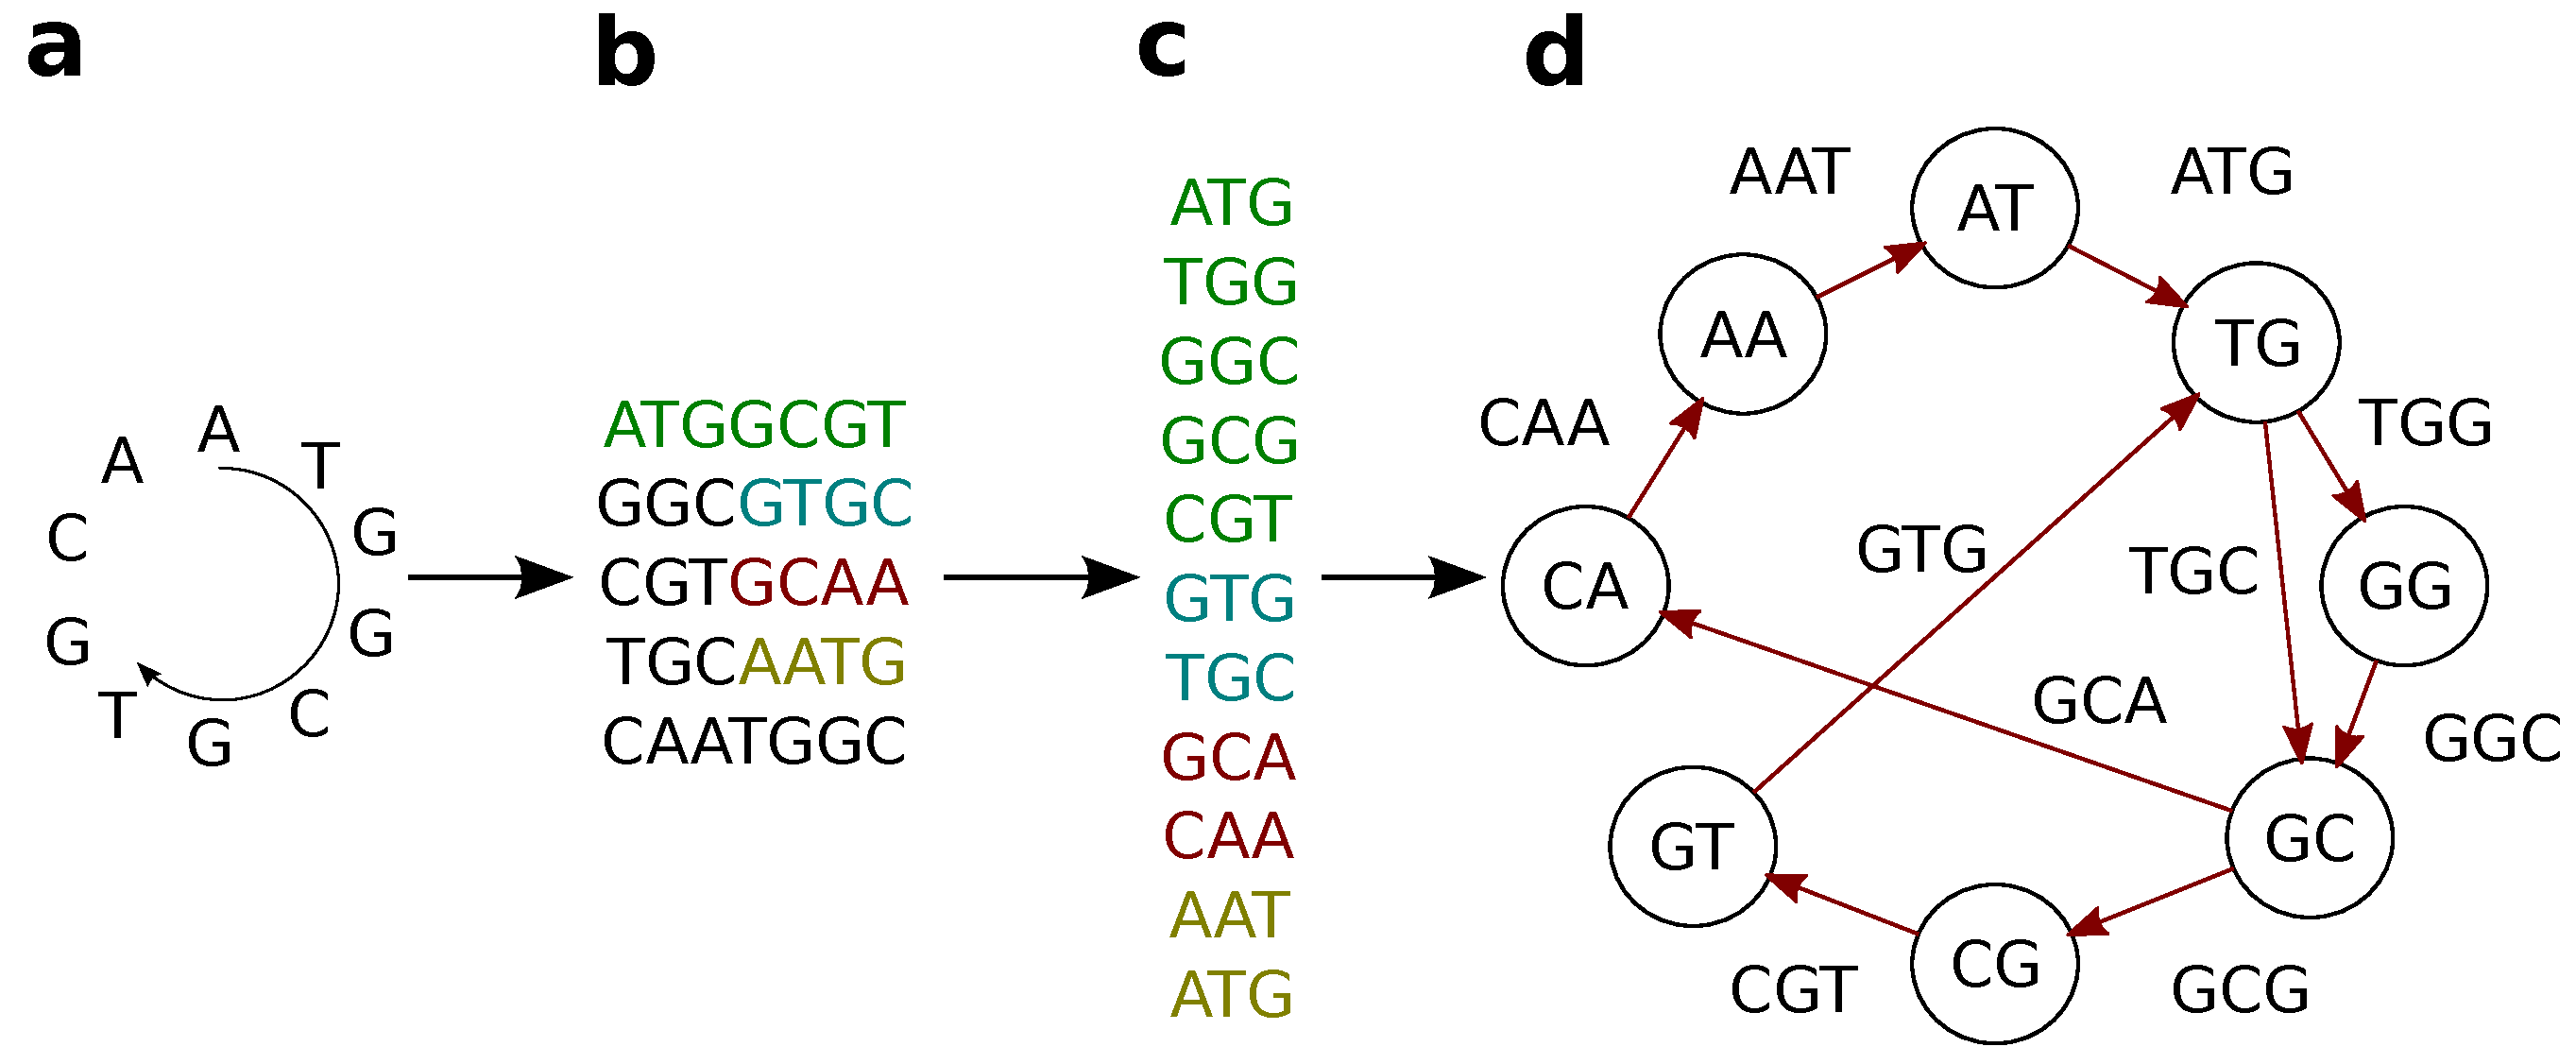
\includegraphics[width=0.8\textwidth]{illumina/de_bruijn.pdf}}
\caption{De Bruijn graph assembly from $k$-mers. (A) A small, circular genome (B) Some short reads sequences. (C) Breaking the reads into $k$-mers ($k = 3$). $k$-mers are coloured according to the sequence from which they are derived. (D) Constructing a De Bruijn Graph from the $k$-mers.}
\label{fig:de-bruijn}
\end{figure*}

Even using the most sophisticated assemblers, it is rare for the entire genome to be recovered as a single, contiguous unit. Consequently, assembly is typically a two-stage process. First, long contiguous sections, named contigs, are constructed. Second, once the contigs cannot be extended any further, ``scaffolding" algorithms~\cite{hunt2014} attempt to join multiple contigs, using insert size information to determine contig order and approximate gap size.

One important challenge that is not resolved by de Bruijn graph assembly is the disambiguation of repeats -- sequences found in multiple places in the genome -- which tangle the de Bruijn graph (Fig.~\ref{fig:tangle}): certain $k$-mer sequences, corresponding to the start and end of repeat regions, have multiple entry and exit paths, the ordering of which cannot be determined. Repeat disambiguation is a major challenge for correct \textit{de novo} assembly. Consequently, several alterations to the sequencing methodology have been developed to provide more data about the positioning of repeat sequences within a genome. 

\begin{figure*}
\centerline{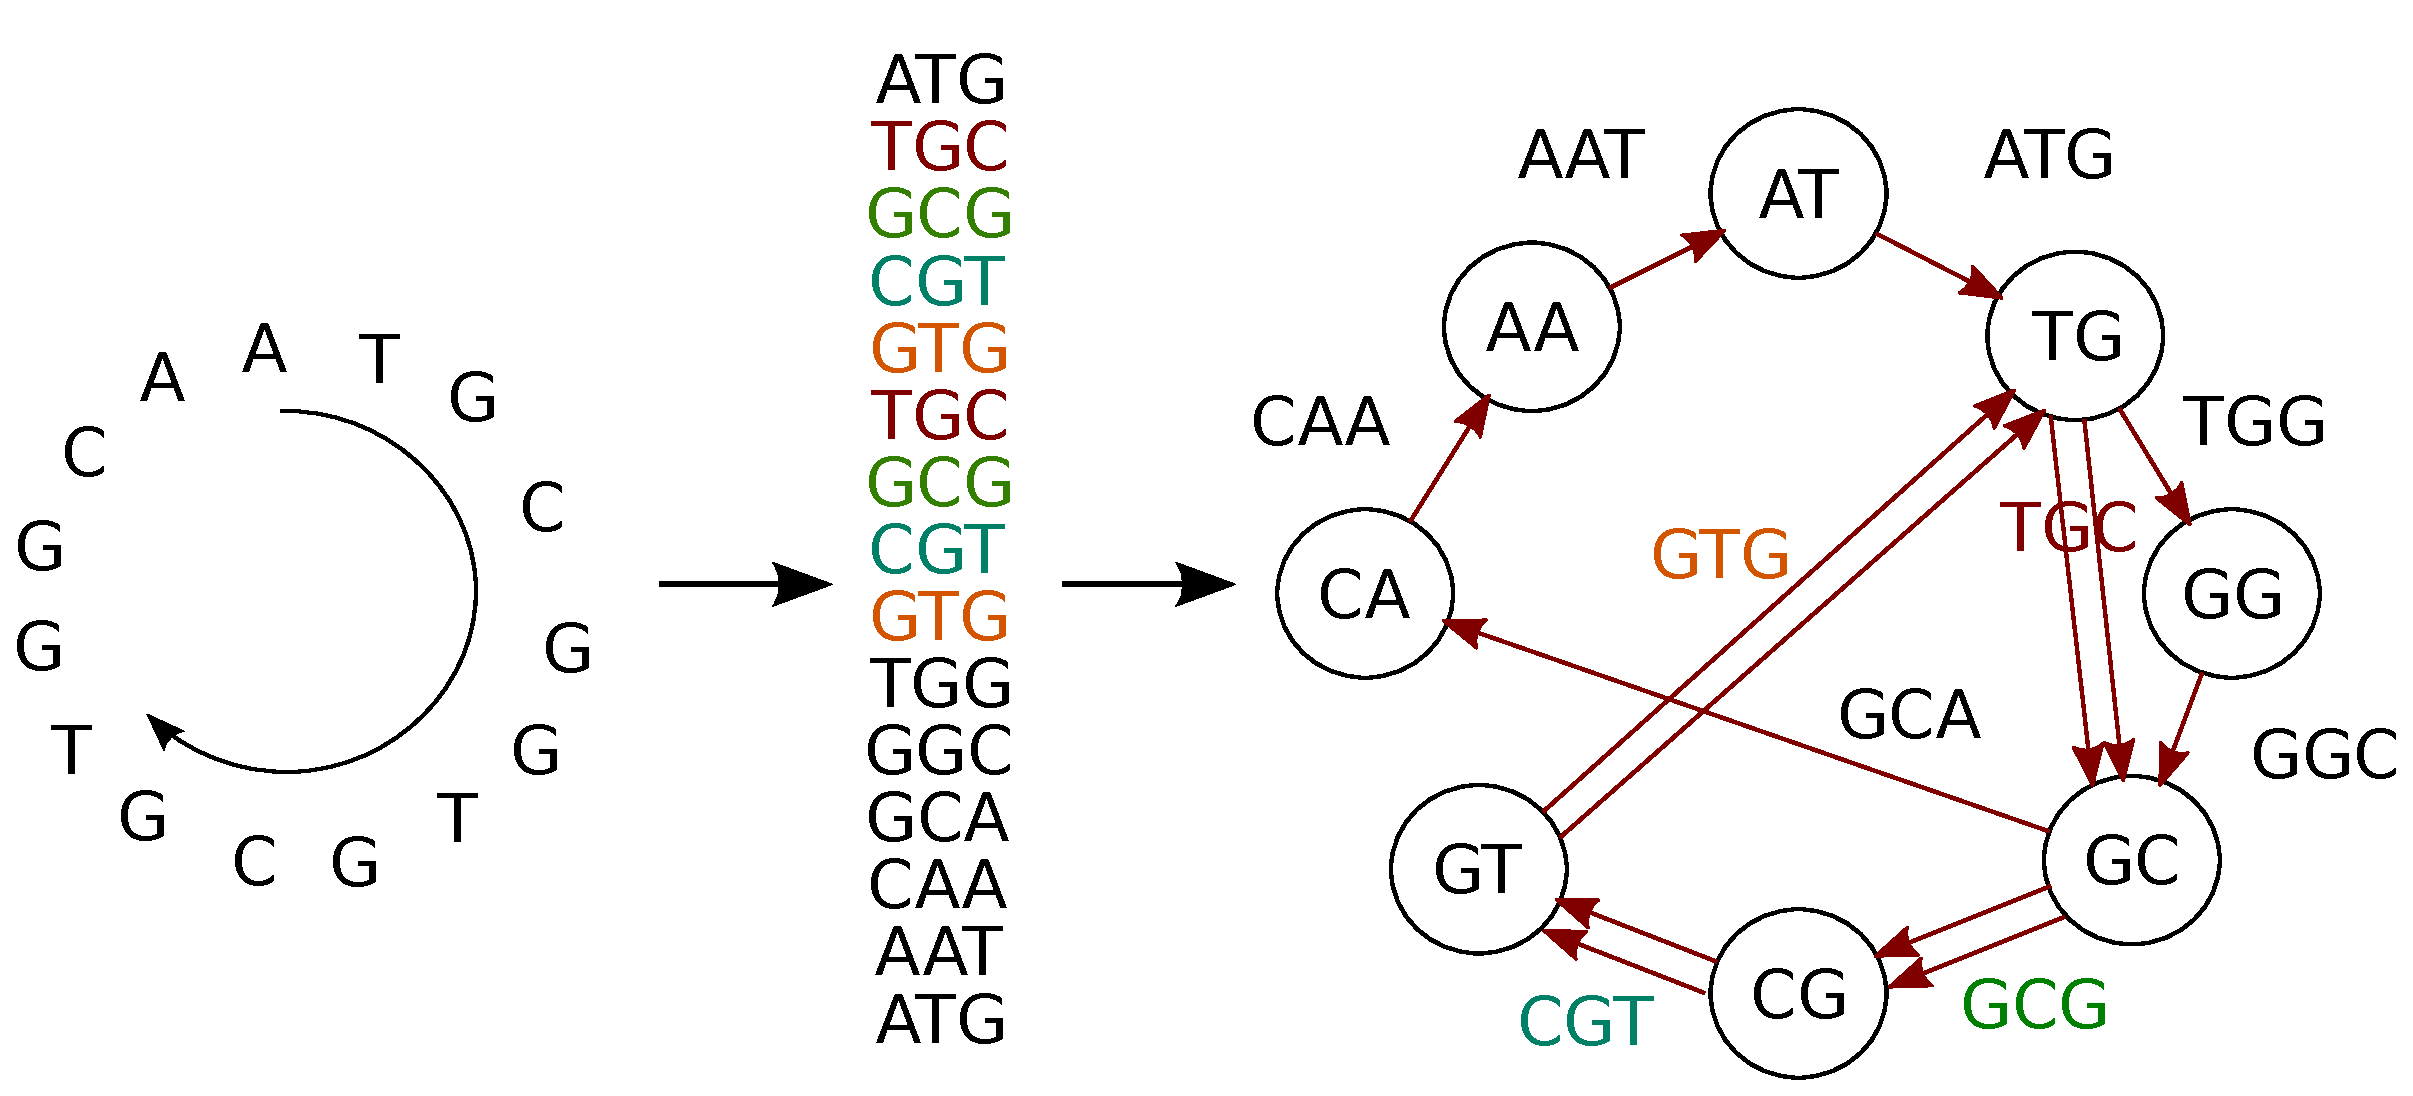
\includegraphics[width=0.8\textwidth]{illumina/de_bruijn_tangle.pdf}}
\caption{A se Bruijn graph with repeats. The larger circular genome ATGCGTGCGTGGCA contains the repeated section TGCGTG, resulting in several 3-mers (TGC, GCG, CGT and GTG, coloured red, green blue and orange respectively) appearing more than once. This results in a tangled de Bruijn graph.}
\label{fig:tangle}
\end{figure*}

\subsection{Paired End Reads and Mate Pair Sequencing}
\paragraph{Paired End and Single End Reads}
The description of \textit{de novo} assembly given above has assumed that reads are ``single-end" -- that is, the fragments of genomic DNA attached to the flowcell surface are sequenced using one strand only. However, a simple modification to the protocol additionally allows sequencing of the complementary strand. This provides two sequences, corresponding to the two ends of the genome fragment, separated by some unsequenced central region. These two sequences can be matched~\cite{edwards1990}, to give a pair of reads (a read pair), separated by some small distance within the genome. The genomic distance from the start of one read to the end of the other is termed the insert size. The genomic libraries used for this paired end sequencing typically contain fragments with an insert size of around 500 bases in length, although this can be controlled during library preparation.

When the insert size (fragment length) is longer than the length of a repeat unit, paired end reads provide extra information that can help to disentangle a de Bruijn graph. By creating a bridge between the start and end sections of a repeat unit, the paired end reads can enable the order of repeat sections to be determined. Some assemblers~\cite{medvedev2011, Bankevich2012} directly incorporate pairing information into the de Bruijn graph; in other assembly pipelines, pairing information is used in the subsequent  scaffolding step to order determine the correct ordering of the contigs.  

\paragraph{Mate Pair Sequening}
Many repeat regions are larger than the average insert size of a paired end library, with the result that fully constructing a genome from short reads is still not possible. To enable further disambiguation of the repeat structure, protocols to create read pairs with a much larger insert size have been developed~\cite{nextera2012}, allowing construction of libraries containing fragments that are several kilobases (kb) in length. These ``mate pair" libraries can be used either alone, or in combination with a paired end library, to provide additional information for a \textit{de novo} assembly.

\subsection{Evaluating Assembly Quality}
Many assemblers incorporate mate pair insert size information into either both the contig assembly and scaffolding processes~\cite{medvedev2011, Bankevich2012}, or just into the scaffolding step~\cite{Zerbino2008} but errors can still occur. These errors can significantly affect the quality of the assembled genome, with repercussions for downstream research. Consequently, error correction and quality evaluation of \textit{de novo} assemblies are problems receiving considerable research interest.

The most serious mistakes found in a \textit{de novo} assembly are large scale scaffolding or extension errors (Fig.~\ref{fig:NxRepair} (A)), in which two two disparate regions of a genome are incorrectly joined together. Similarly, large insertion or deletion errors (indels) create structural irregularities in the \textit{de novo} assembly; whereas mistakes in base calling lead to errors at a single position only. 

The most common method of evaluating assembly quality is to measure its $N50$ score, defined as ``the length of the shortest contig in the set that contains the fewest (largest) contigs whose combined length represents at least 50\% of the total assembly"~\cite{Miller2010}. However, this evaluation method optimises only for contig length, without considering the correctness of the assembly. When a reference genome is available, the modified $NA50$ statistic~\cite{Gurevich2013} can be used, which considers only contig sections that correctly align to the reference. Recent work, such as the Assemblathon~\cite{Bradnam2013} and GAGE~\cite{Salzberg2012} collaborations used this metric to compare the quality of the \textit{de novo} assemblies prepared by various assemblers by comparing them with their equivalent reference genomes. However, in the absence of a high-quality reference genome, other methods of quality evaluation must be used.

\subsection{Error Detection Methods}
Ghodsi et al.~\cite{Ghodsi2013} have developed a Bayesian method of assembly quality evaluation, which can calculate an assembly quality score, without requiring a reference genome. However, this provides only an overall quality score and cannot be used to identify errors or low-quality regions. Several recent papers have developed error identification and correction methods, which perform a fine-grained analysis of assembly quality. The most well-known of these is the A5 Assembly Pipeline~\cite{Coil2014, tritt2012}, which includes an error detection and rescaffolding step that makes use of mate pair alignment information. Two new tools, REAPR~\cite{Hunt2013} and ALE~\cite{Clark2013} have also been developed to use read pair data to identify misassemblies. A similar tool is currently under development at the Broad Institute~\cite{pilon2014}. However, with the exception of ALE, which is no longer actively maintained, these newer tools are not optimised to use mate pair information.  

This chapter describes NxRepair, an assembly error detection tool that we designed to identify the most serious misassemblies by examining the distribution of Nextera mate pair insert sizes. NxRepair does not require a reference genome and can be used with assemblies prepared with a single mate pair library alone. It specifically targets the most serious scaffolding errors and large-scale indels by identifying regions with a high number of anomalous insert sizes, or very few supporting reads, breaking the scaffold and optionally trimming out the misassembled region. NxRepair also provides a fine-grained quality score, allowing researchers to visualise poor-quality regions. 

In the following sections, we describe the theoretical basis of NxRepair and its efficient implementation using an interval tree data structure. We then demonstrate the use of NxRepair on bacterial genomes assembled from a single Nextera mate pair library. For the \textit{de novo} assembly process, we use the state of the art SPAdes assembler~\cite{Bankevich2012}, which explicitly uses insert size information during contig construction, as well as for scaffolding. Using these genomes, we benchmark NxRepair against the error correction module of the A5 assembler, A5qc~\cite{tritt2012}, which is currently the most widely used error correction tool, demonstrating NxRepair's superior performance. We conclude the chapter with a discussion of the performance and limitations of NxRepair as a quality control tool and discuss possible extensions that could improve performance.

\begin{figure*}
\centerline{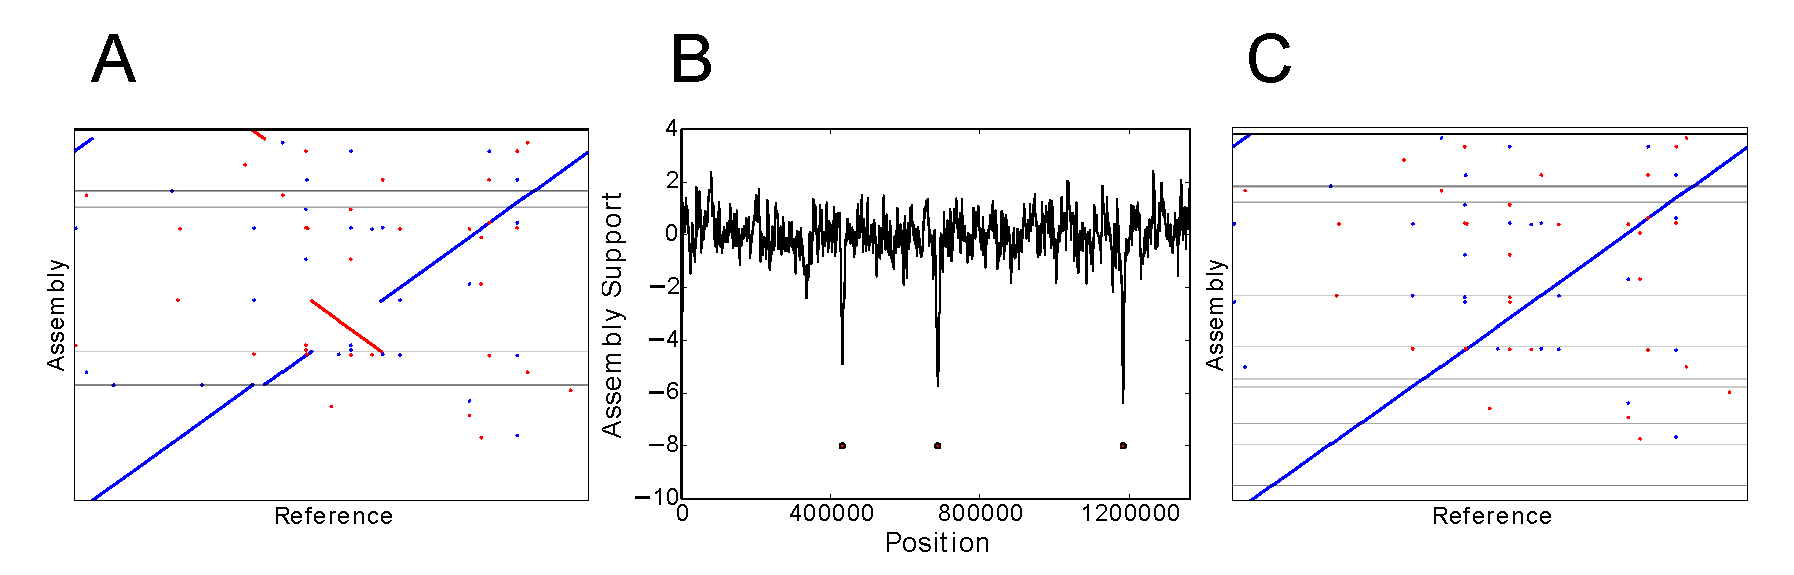
\includegraphics[width=0.8\textwidth]{illumina/fig1_nxrepair.pdf}}
\caption{Using NxRepair to remove large misassemblies. (A) Alignment of the \textit{de novo} assembly of the M. tuberculosis genome to its reference genome. The assembly contains several large misassemblies. (B) A plot of NxRepair's support metric against scaffold position for the assembly. Low support for the assembly is identified in three regions of a contig. (C) Breaking the contigs at the identified positions resolves the most significant misassemblies. In (A) and (C), horizontal lines demarcate the scaffold boundaries.}\label{fig:NxRepair}
\end{figure*}

\clearpage

\section{Theory}
\subsection{Statistical Analysis of Mate Pair Insert Sizes}
\label{sect:illumina_theory}
Nextera mate pair libraries are prepared to have a certain insert size, typically between 1 and 10 kb. Following construction of a \textit{de novo} assembly, it is possible to align the mate pair reads used to construct the assembly back to the assembly itself. The actual distance along the \textit{de novo} assembly between the two reads that form a mate pair can then be calculated. Large-scale errors in the assembly will cause mate pair reads aligning near to the error to have unusual insert sizes and read orientations. This means that we can use the insert size distribution displayed by mate pair reads aligning at different sites along the assembly to evaluate the local assembly quality. We identify assembly errors at sites where the local insert size distribution deviates too far from that observed in the rest of the genome.       

We model the observed insert sizes of mate pairs aligned to the \textit{de novo} assembly using a two-component mixture distribution. The first component of this mixture is the insert size distribution of correctly aligned mate pairs.  We model the distribution of insert sizes, $Y$, as a normal distribution with mean $\hat{\mu}$ and standard deviation $\hat{\sigma}$: $Y \sim N(\hat{\mu},\hat{\sigma}^2).$ We estimate $\hat{\mu}$ and $\hat{\sigma}$ for the entire genome by aligning reads back to the assembly and using robust estimators (see below). The second component, defined as a uniform distribution across the contig size $U(0,L)$ for a contig of length $L$, captures anomalous insert sizes. 

To calculate the degree of support for the assembly at each site across a contig, NxRepair retrieves all mate pairs spanning the region $[i-W, i+W]$, of size $2W-1$ at position $i$ on the contig, where spanning is defined to mean that one read ends entirely before the region $[i-W, i+W]$ and the other read begins entirely after (see Fig.~\ref{fig:spanning}.) The default value of $W$ is 200 bases (see Table~\ref{tab:parameters}). 

A uniform distribution was selected to model anomalous insert sizes, as it makes no assumption about the cause of an anomaly. It is uniform over the contig length, $L$, as opposed to over all possible sites in the assembly, as only pairs where both members align fully to that contig are considered. Similarly, even though the insert size distribution for correctly aligned mate pairs will typically display a longer tail than the normal distribution (unless a gel-extraction protocol is used), we found that using a normal distribution to model correct insert sizes did not adversely affect NxRepair's error detection. This is because each site is spanned by many mate pairs and the insert size of correctly aligned mate pairs is not correlated with location. Consequently, despite these assumptions, the small fraction of correctly aligned mate pairs with a very large insert size do not lead to false positives in error identification. 

We define a latent indicator variable $X_l\in\{0,1\}$ for each pair of reads, $l$, which takes the value $1$ if the insert size came from the null distribution, and $0$ otherwise. Within each window queried, the probability that each retrieved read, $r_l$ is drawn from the null distribution is given by:

\begin{eqnarray} P(X_l=x|Y_l)& =& \frac{\pi_x(Y_l|X_l=x)}{\sum_{k=0}^1 \pi_k(Y_l|X_l=k)}
\label{eq:posterior}  
\end{eqnarray}

where $Y_l$ is the insert size of read pair $l$, $\pi_k$ is the user defined prior probability of class $k$ and $\pi_1 + \pi_0 = 1$. The default value of $\pi_0$ is 0.01 (see Table~\ref{tab:parameters}), meaning that in the absence of any insert size information, 99 \% of read pairs are expected to arise from the null distribution.  

Within each window, the total support, $D_i$ for a correct assembly at position $i$ can be calculated as:

\begin{equation}
D_i = \sum_{l=1}^N P(X_l=1|Y_l)\cdot C_l
\end{equation}

where the summation is over all read pairs aligning across position $i$ and $C_l$ is an indicator variable, reporting pairing orientation:

\begin{equation}
    C_l=
    \begin{cases}
      1, & \text{if}\ \text{mate pairs have correct orientation and strand alignment} \\
      0, & \text{otherwise}
    \end{cases}
  \label{eq:C}
  \end{equation}

Within each contig, the contig assembly support mean $\mu_D$ and variance $s_D$ are calculated from all reads aligning to the contig,
\begin{equation}
\mu_D = \frac{\sum_{l=1}^N D_l}{N} \qquad s_D = \frac{\sum_{l=1}^N \sqrt{(D_l - \hat{\mu})^2}}{N}
\label{eq:contigD}
\end{equation}

We use these contig specific mean and variance, rather than the global values, to prevent local variations in coverage from either causing false positives or masking changes in the insert size distribution. Using these values, we calculate the Z-score $z_l$ within each queried interval as: 

\begin{equation}
z_l = \frac{D_l - \hat{\mu}_D}{s_D}
%\hat{\mu} = \frac{\sum_l^N D_l}{N} \qquad \s = \frac{\sum_l^N \sqrt{(D_l - \hat{\mu})^2}}{N}
\label{eq:zscore}
\end{equation}

The Z-score is sensitive both to local changes in the insert size distribution, and to large variations in the number of correctly aligned mate pairs, for example caused by a large number of reads with a mate aligning to a different contig. This ensures that NxRepair can identify misassemblies occurring both within and between contigs.  

A misassembly is identified if $z_l < T$ for a user-defined threshold $T$ (default value -4). This threshold describes the number of standard deviations below the mean assembly support that is required to identify an anomaly. The default value of -4 will flag only positions whose assembly support is less than four standard deviations below the mean level of support. Optimisation of the default threshold value is described in Section~\ref{sect:optimisation}

\begin{figure}
\centerline{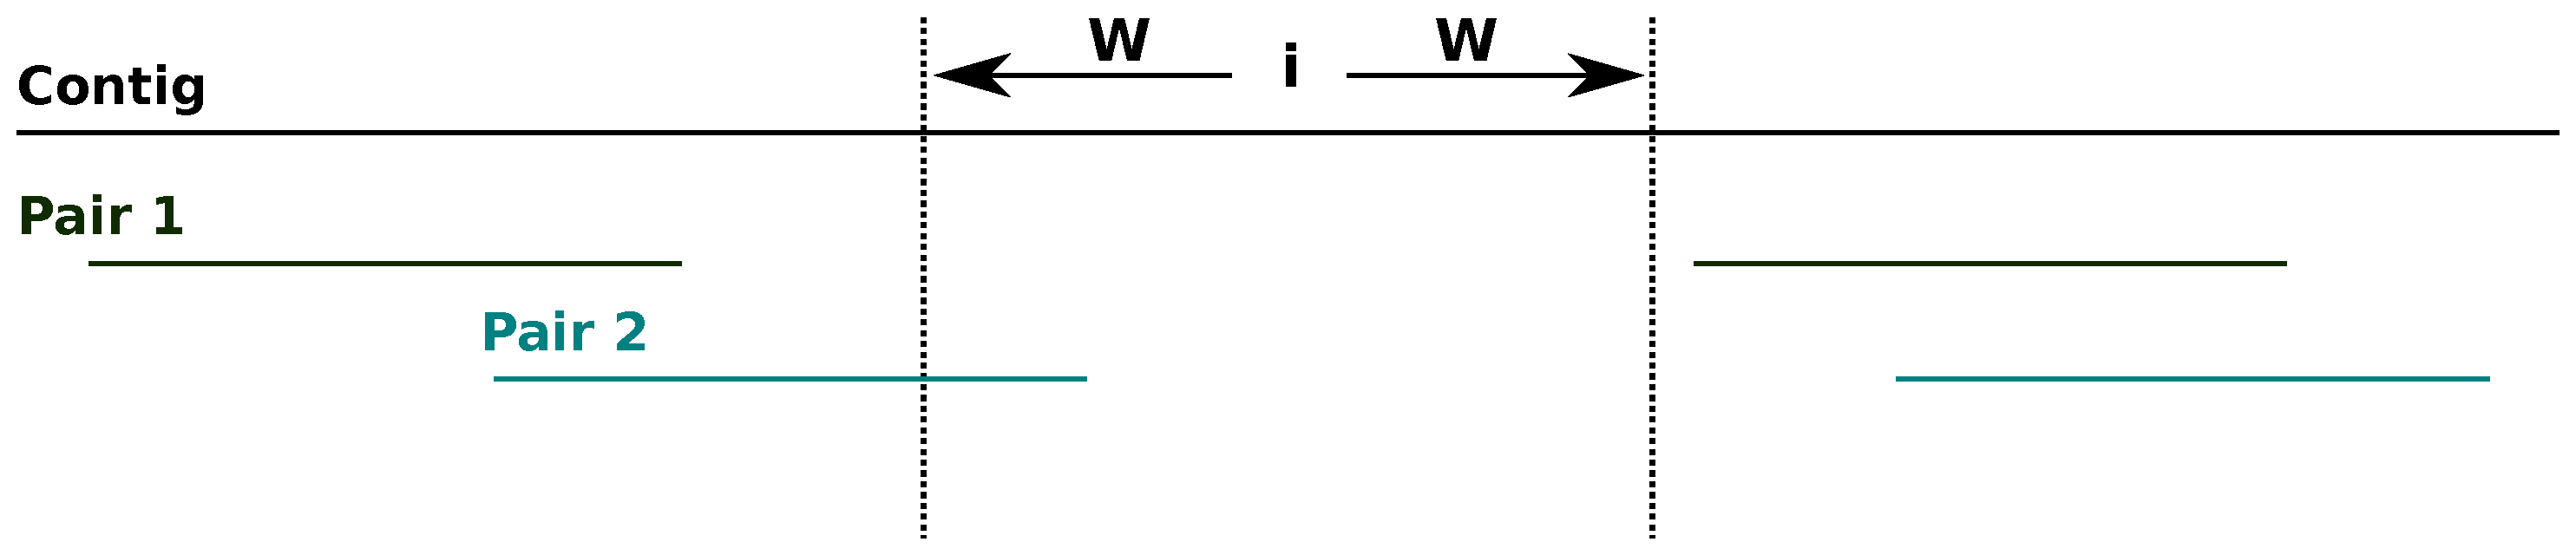
\includegraphics[width=0.8\textwidth]{illumina/spanning.pdf}}
\caption{Schematic illustrating mate pairs spanning a selected region. The upper read pair (green) spans the indicated region, as both reads align entirely outside of the region $[i-W, i+W]$. The lower read pair (cyan) do not span the indicated region, as the left-hand read overlaps the target area. \label{fig:spanning}}
\end{figure}

\subsection{Global Assembly Parameters}
NxRepair identifies misassemblies by identifying regions where the mate pair insert size distribution differs significantly from the insert size distribution across the entirety of the \textit{de novo} assembly. Consequently, it is necessary to have a robust estimate of the global mate pair insert size distribution. For calculation of population statistics, mate pairs that align to different contigs are excluded, as are mate pairs with an incorrect strand or pairing orientation and pairs whose insert size exceed 30 kb (approximately 10 times the mean insert size). Pairs whose mapping quality falls below a user specified threshold (minmapq, default value 40) are also excluded, removing reads that are not uniquely mapped from the calculation of global parameters. The global mean $\hat{\mu}$ and median absolute deviation ($\text{MAD}$) are calculated across all contigs in the assembly as:

\begin{equation}
\hat{\mu} = \frac{\sum_{l=1}^N Y_l}{N} \qquad \text{MAD} = \text{median}_m(|Y_m - \text{median}_l(Y_l)|)
\label{eq:global}
\end{equation}

where $\text{median}_l(Y_l)$ is the median insert size of reads with correct pairing behaviour and $|Y_m - \text{median}_l(Y_l)|$ is the absolute value of the residual from the median of the $m$th on $N$ reads. The standard deviation, $\hat{\sigma}$, was then calculated by scaling the MAD using:

\begin{equation}
\hat{\sigma} = K \cdot \text{MAD}
\label{eq:mad_to_sigma}
\end{equation}

where 

\begin{equation}
K = \frac{1}{\frac{3}{4} \cdot \phi^{-1}} \sim 1.4826
\label{eq:k_scale}
\end{equation}

and $\phi^{-1}$ is the quantile function~\cite{Leys2013}

The $\text{MAD}$ is a robust estimator for the standard deviation, as it is not sensitive to outliers, such as the long tail of the mate pair insert size distribution. Using the MAD as an estimator prevents over-estimating the variance of the insert size, allowing anomalously large insert sizes to be correctly identified.

These were then used as the parameters of the null distribution, as described above (Section~\ref{sect:illumina_theory}).

\subsection{Interval Tree Construction}
To facilitate rapid lookup of mate pair properties, we construct an interval tree~\cite{cormen2009} for each contig in the \textit{de novo} assembly. An interval tree is a data structure that facilitates $O(\text{log} n + m)$ lookup of intervals that span a given point or interval, for $n$ total entries and $m$ spanning entries. The interval tree contains the start and end positions of each mate pair aligned to that contig, as well as a flag variable indicating whether that mate pair had correct strand and pairing orientation. Mate pairs where the two reads align to different contigs were excluded. Mapping quality is currently not considered at this stage - reads are retained regardless of the mapping quality (mapq) score. For each position $i$ for which the Z-score is to be calculated, the tree is queried with a start position $i-W$ and end position $i+W$, to retrieve read pairs spanning the interval between positions $i-W$ and $i+W$ (exclusive). The insert sizes of retrieved read pairs are then used to calculate the Z-score for position $i$. This allows NxRepair to rapidly query positions across a contig to discover the insert size distribution at the queried position. Use of the interval tree significantly increases the efficiency of Z-score calculation, as each pair of reads is fetched only once in order to build the tree. All relevant parameters are then stored in the tree for rapid look-up when a position is queried. This has several advantages. Firstly, it is significantly faster than fetching reads only when a position is queried. Secondly, it is more space efficient than a frequency array of all positions on all contigs but does not lose any information about the exact alignment positions. Finally, once construction of the tree is complete, multiple passes across a contig (for example with different spatial resolutions, or using different window sizes) can rapidly be made using the same tree.      

\subsection{Misassembly Location and Contig Breaking}
To improve the quality of the \textit{de novo} assembly, once a misassembly has been located, a contig is broken into two separate pieces at the site of a misassembly. The broken ends of the two new contigs can optionally be trimmed by a user defined length (default 4 kb) to remove the misassembled region. Trimming allows removal of the incorrectly assembled regions around a break-point, but can be switched off if a user does not want any sequence to be removed from the assembly. To prevent excessive clipping, misassemblies separated by less than the trimming distance are grouped together, the contig is broken at the start and end of the misassembled region and the misassembled section is discarded. Low-scoring regions within the trimming distance of the ends of contigs are not considered misassemblies, as the high proportion of mate pairs aligning here whose mate maps to a different contig reduces the number of pairs under consideration and hence lowers the observed Z-score. This also ensures that circular molecules, such as small plasmids, which are assembled into a single contig, are not truncated because of mate pairs at either end of the assembly that appear to span the entire contig, but which are spatially close when circularisation is considered.

\subsection{Availability and Dependencies}
NxRepair is available for free anonymous download from the Python Package Index (PyPI) here: \url{https://pypi.python.org/pypi/nxrepair}.
The source code, written in python is hosted on GitHub: \url{https://github.com/rebeccaroisin/nxrepair}.
A full tutorial and API can be found on ReadTheDocs: \url{http://nxrepair.readthedocs.org/en/latest/}.

NxRepair makes use of several further open source libraries, specifically:

\begin{itemize}
\item[] Numpy~\cite{numpy} (\url{http://www.numpy.org/})
\item[] Scipy~\cite{scipy} (\url{http://www.scipy.org/})
\item[] Matplotlib~\cite{Hunter2007} (\url{http://matplotlib.org/})
\item[] Pysam (\url{https://pypi.python.org/pypi/pysam}), the python wrapper for Samtools
\item[] Samtools~\cite{li2009} (\url{http://samtools.sourceforge.net/})
\end{itemize}

We installed the numpy, scipy and matplotlib libraries via Anaconda (\url{https://store.continuum.io/cshop/anaconda/}).

We have used the Interval Tree implementation from the bx-python library (\url{https://bitbucket.org/james_taylor/bx-python/wiki/Home}).   

\section{Experimental Methods}
\subsection{Data}
\textit{Preparation of the genome libraries was carried out by Emma Carlson and Niall Gormley at Illumina Cambridge.} \\
Nine bacterial genomes were prepared according to the Nextera mate pair protocol and sequenced in duplicate in a single MiSeq run using $2 \times 151$ bp reads. The organisms sequenced are shown in Table~\ref{data-description}. Reads were trimmed using the MiSeq inbuilt trimmer. Table~\ref{tab:yield} gives an overview of sequencing yield, mean quality and read length after trimming. The untrimmed reads are available from BaseSpace via \url{https://basespace.illumina.com/s/TXv32Ve6wTl9}. In addition,
the trimmed reads are available at the European Nucleotide Archive (ENA) at \url{http://www.ebi.ac.uk/ena/data/view/PRJEB8559}. Note that only these Nextera mate pair libraries were used. No additional single end or paired end libraries were required. For performance optimisation, the first replicate from each genome sequenced was used as a training set. The test set, for performance evaluation, was formed from the second replicate of each genome. 

\subsection{Performance Optimisation}
\label{sect:optimisation}
\paragraph*{ROC Plots}
To optimise the threshold in the Z-score, $Z$, below which to identify a misassembled region, we prepared ROC plots using Replicate 1 of each genome, varying the threshold value, $T$, in steps of 1 between -10 and 0. 

The positions of true misassemblies were identified by aligning each \textit{de novo} assembly to its reference genome using QUAST~\cite{Gurevich2013}. To correctly compare the sites of true misassemblies with those identified by NxRepair, we divided each contig of the assembly into short stretches of 1 kb length. We then prepared an array, $A_{Nx}$ of size $\frac{L}{1000}$ for contig length $L$, corresponding to misassemblies identified by NxRepair. $A_{Nx}$ was filled as follows:

\begin{equation}
    A_{Nx}=
    \begin{cases}
      1, & \text{if}\ \text{NxRepair identified a misassembly in stretch $i$} \\
      0, & \text{otherwise}
    \end{cases}
  \label{eq:found}
\end{equation}

To prepare the ROCs, each position $i$ in $A_{Nx}$ was labeled as true positive (TP) if $A_{Nx}[i] = 1$ and a true misassembly fell within it, true negative (TN) if $A_{Nx}[i] = 0$ and no true misassembly occurred within the interval, false positive (FP) if $A_{Nx}[i] = 1$ but no true misassembly had occurred, or false negative (FN) if $A_{Nx}[i] = 0$ but the interval contained a true misassembly. The 1 kb interval used was the same interval used in error identification, ensuring that the resolution of the evaluation matched the error detection resolution. The true positive rate (TPR) and false positive rate (FPR) were then calculated as follows:

\begin{equation}
\text{TPR} = \frac{\text{TP}}{\text{TP} + \text{FN}} \qquad \text{FPR} = \frac{\text{FP}}{\text{FP} + \text{TN}}
\label{eq:tpr}
\end{equation}

Based on the resultant ROC plots, shown in Fig.~\ref{fig:ROCs}, a threshold in $Z$ of -4 was found to detect true misassemblies with minimal false positives, so was used for all subsequent analyses. 

\begin{figure}
\centerline{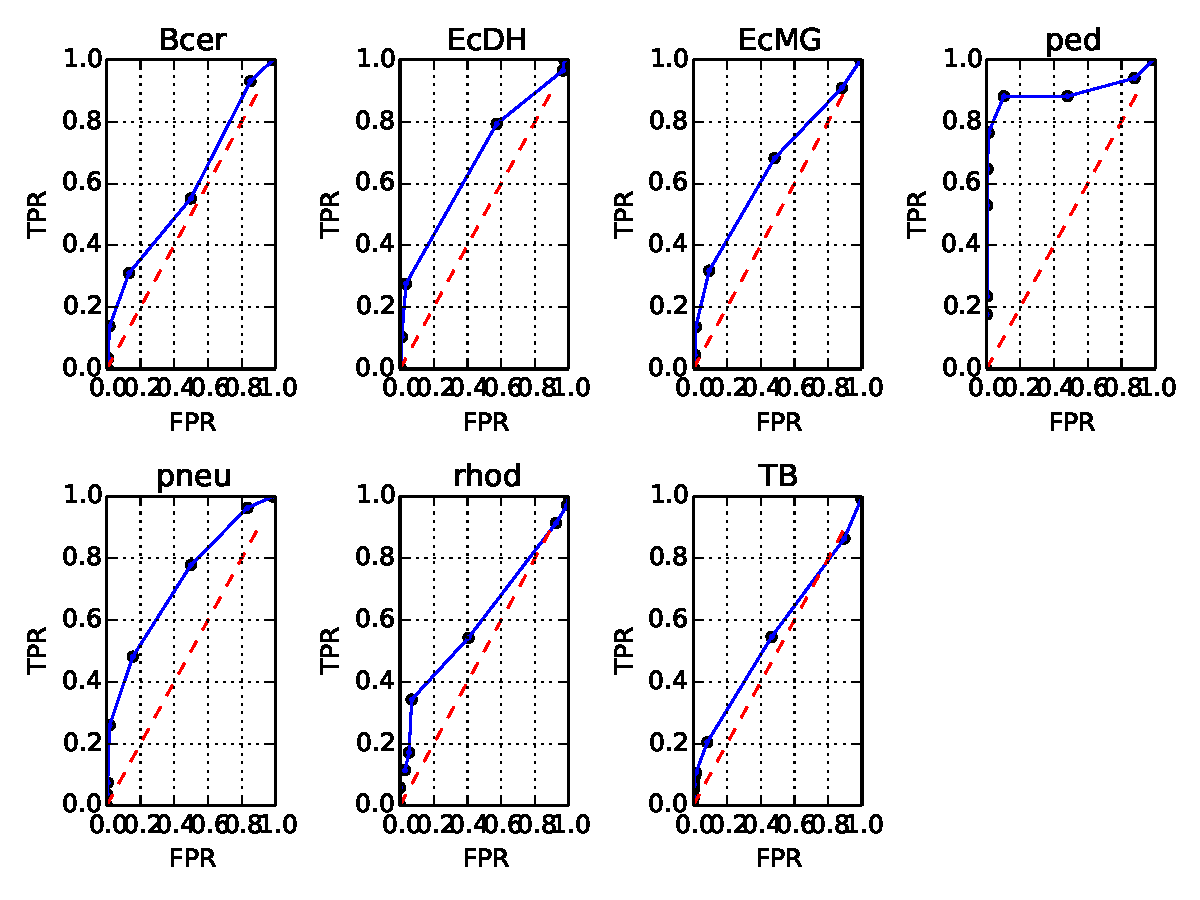
\includegraphics[width=0.8\textwidth]{illumina/allROC.pdf}}
\caption{ROC plots for the seven genomes containing misassemblies. Each plot is labelled with an abbreviation of the genome used. The correspondence between the abbreviation and the bacterial genome is shown in Table~\ref{data-description}. ROC plots for the List. and Meio. genomes are not shown, as these did not contain any large misassemblies in the original assembly. \label{fig:ROCs}}
\end{figure}

\paragraph{Profiling}
Performance analysis was performed on a single core with 8 GB RAM available. Runtime analysis was performed using the python cProfile module. The memoryprofiler python module was used to analyse memory usage.

\subsection{Workflow Pipeline}
\textit{De novo} assemblies were prepared using the SPAdes Assembler, version 3.1.1~\cite{Bankevich2012}:

\texttt{spades.py -k 21,33,55,77 -t 4 \\ --hqmp1-12 bacteria.fastq.gz  --hqmp1-fr -o assembly}

The initial assembly quality was evaluated using QUAST~\cite{Gurevich2013} (version 2.3, see~\url{http://bioinf.spbau.ru/quast}) to align the \textit{de novo} assembly to a reference genome:

\texttt{python quast.py -o results\_sample -t 16 \\  -R ref/reference.fna sample\_new.fasta }

  Following assembly, the same reads used to generate the assembly were aligned back to the \textit{de novo} assembly using BWA-MEM~\cite{li2013} (BWA version 0.7.10). A sorted BAM file of the resulting alignment was then prepared using SAMtools (version 1.1)~\cite{li2009}: 

\texttt{bwa index sample/scaffolds.fasta}

\texttt{bwa mem sample/scaffolds.fasta -p bacteria.fastq.gz | samtools view -bS - |  samtools sort - sample}

\texttt{samtools index sample.bam}

We identified misassemblies using NxRepair (version 0.13) as follows:

\texttt{python nxrepair.py sample.bam   sample/scaffolds.fasta sample\_scores.csv  sample\_new.fasta -img\_name sample\_new}


The default parameters used and their meanings are shown in Table~\ref{tab:parameters}. These have been optimised for Illumina Nextera mate pair libraries with a mean insert size of approximately 4 kb. For mate pair libraries with a much larger (smaller) insert size, the maxinsert and trim parameters may need to be increased (decreased).

\begin{table}
\begin{center}
\caption{NxRepair Parameters. This table lists the user-modifiable parameters used in NxRepair, along with the default values used and a brief description of the meaning of each parameter. \label{tab:parameters}}
\begin{tabular}{llp{8cm}}
    \hline
    Parameter & Default Value & Meaning \\ \hline
    imgname & None & Prefix under which to save plots. \\
    maxinsert & 30000 &  Maximum insert size, below which a read pair is included in calculating population statistics.\\
    minmapq & 40 & Minimum MapQ value, above which a read pair is included in calculating population statistics.\\
    minsize & 10000 & Minimum contig size to analyse.\\ 
    prior & 0.01 & Prior probability that the insert size is anomalous.\\
    stepsize & 1000 & Step-size in bases to traverse contigs.\\
    trim & 4000 & Number of bases to trim from each side of an identified misassembly.\\
    T & -4.0 & Threshold in Z score (number of standard deviations from the mean) below which a misassembly is called.\\
    window & 200 & Window size across which bridging mate pairs are evaluated.\\ \hline
\end{tabular}
\end{center}
\end{table}

Finally we used QUAST~\cite{Gurevich2013} to evaluate the assembly quality following NxRepair by aligning the \textit{de novo} assembly to a reference genome as described above.


\section{Results}
We used NxRepair to correct \textit{de novo} assemblies from Replicate 2 of each of the nine bacterial genomes described above. Mate pair reads were trimmed, assembled using the SPAdes assembler (version 3.1.1)~\cite{Bankevich2012} and then aligned back to the assembled scaffold using BWA-MEM~\cite{li2013}. We used QUAST~\cite{Gurevich2013} to evaluate the assembly quality before and after NxRepair correction by aligning to an appropriate reference genome. For all NxRepair analyses, the default parameters, shown in Table~\ref{tab:parameters} were used. Fig.~\ref{fig:NxRepair} (A) shows a misassembled genome that contained several scaffolding errors identified by NxRepair (Fig.~\ref{fig:NxRepair} (B)). Following NxRepair correction, the most significant structural misassemblies were resolved (Fig.~\ref{fig:NxRepair} (C)). The improvement following NxRepair correction is shown for all nine genomes in Table~\ref{tab:improvement} (middle column). For two assemblies, errors were removed without reducing NGA50; for one genome, errors were removed but NGA50 was slightly reduced; for six genomes, three of which contained no large errors, no errors were found and the assembly was unchanged. We are not able to correct all misassemblies, as not all misassemblies exhibit a change in Z-score large enough to identify an error against the background score fluctuation caused by the wide insert size distribution of the Nextera mate pairs. 

To benchmark NxRepair's performance, we also attempted to identify assembly errors using the A5qc error correction module of the A5 Assembly pipeline~\cite{tritt2012}. The results are shown in Table~\ref{tab:improvement} (right hand column). For eight of the nine genomes evaluated, A5qc was unable to detect any errors. For the final genome (K. pneumoniae), A5qc did detect errors, but the contig-breaking process left Quast unable to align the resultant assembly to the reference genome. Re-scaffolding using the A5 scaffolder did allow reference alignment, but the assembly contained more misassemblies (15) than the original assembly. Consequently, we are confident that, for these high-quality alignments, NxRepair is a superior error-detection tool. 

Despite this good performance, it is clear that NxRepair is not able to find all misassemblies present. There are several reasons for this. Firstly, NxRepair's resolution is limited to relatively large-scale errors, as a very large disruption in mate pair insert sizes over a region of approximately 1 kb to significantly reduce the Z-score. Consequently, indel errors with a displacement smaller than 1 kb will not be detected. Secondly, NxRepair is limited by the intrinsic error rate of the mate pair library used. If the insert size distribution has a very wide variance, large fluctuations caused by assembly errors will be masked, making error correction more challenging. 

A number of improvements to NxRepair might mitigate these issues. Firstly, NxRepair currently identifies errors using a simple threshold applied to the total assembly support from spanning mate pairs, $D$. A more rigorous approach would implement a fully probabilistic method of error detection, using the distribution of spanning mate pair insert sizes to evaluate the relative probability of an error. 

Furthermore, NxRepair currently uses a user-defined prior probability of incorrect pairing and uses some simplistic thresholding to determine the parameters of the global insert size distribution. It would be possible to implement simultaneous co-estimatation of the mate pair error rate and the insert size distribution. In addition to relieving the user of estimating the error rate of their mate pair library, this would improve the accuracy of parameter estimation for the correct mate pairs, particularly for libraries with a large mate pair error rate. However, this would not necessarily translate into improved accuracy of error detection, as noise from the mate pair library would still mask true errors.        

\begin{table}[]
\begin{center}
\caption{Number of large misassemblies and NGA50 as reported by QUAST before (left) and after correction by NxRepair (middle) and A5qc (right) for the second replicate of each of the nine genomes analysed using NxRepair. \label{tab:improvement}}
\resizebox{\textwidth}{!}{
{\begin{tabular}{llllllll}\hline
 & & \multicolumn{2}{l}{Before NxRepair} & \multicolumn{2}{l}{{\bf After NxRepair}} & \multicolumn{2}{l}{After A5qc} \\\hline
Genome & Genome size & No. & NGA50 & No. & NGA50 & No. & NGA50 \\\hline
B. cereus ATCC 10987 & 5,432,652 & 0 & 1,157,846 & 0 & 1,157,846 & 0 & 1,157,846 \\
E. coli K-12 substr. DH10B & 4,686,137 & 7 & 573,003 & 6 & 573,003 & 7 & 573,003 \\
E. coli K-12 substr. MG1655 & 4,641,652  & 3 & 693,692 & 3 & 693,692 & 3 & 693,692\\
L. monocytogenes EGDe & 2,944,528 & 0 & 1,496,613 & 0 & 1,496,613 & 0 & 1,496,613 \\
M. ruber DSM 2366 & 4,839,203 & 0 & 2,702,549 & 0 & 2,702,549 & 0 & 2,702,549 \\
P. heparinus DSM 2366 & 5,167,383 & 1 & 1,269,147 & 0 & 952,558 & 1 & 1,269,147 \\
K. pneumoniae MGH 78578 & 5,694,894 & 8 & 578,813 & 8 & 578,813 & - & - \\
R. sphaeroides 2.4.1 & 4,602,977 & 8 & 2,715,434 & 8 & 2,715,434 & 8 & 2,715,434 \\
M. tuberculosis H37Ra & 4,411,532 & 63 & 186,136 & 57 & 186,136 & 63 & 186,136 \\\hline
\end{tabular}}{}
}
\end{center}
\end{table}  


\subsection{Performance}
We evaluated the runtime and peak memory usage of NxRepair on each of the nine genomes analysed. The results are shown in Table~\ref{tab:performance}. The most memory and computationally intensive part of the NxRepair analysis is construction of the interval trees. The size of each interval tree is dependent on the contig size. Consequently, we expect both runtime and memory usage to scale with the size of the largest contig. 

\begin{table}
\begin{center}
\caption{NxRepair performance analysis. The total run-time and memory usage of NxRepair in analysing \emph{de novo} assemblies of each of the nine genomes described in Table~\ref{data-description}. Results are shown for Replicate 1 of each genome. \label{tab:performance}}
\begin{tabular}{lll}
    \hline
    Bacterium & Total Time (s) & Memory Usage (MiB) \\ \hline
    B. cereus ATCC 10987 & 78 & 271 \\
    E. coli K-12 substr. DH10B & 123 & 444 \\
    E. coli K-12 substr. MG1655 & 70 & 260 \\
    L. monocytogenes EGDe & 97 & 383 \\
    M. ruber DSM 2366 & 259 & 565 \\
    P. heparinus DSM 2366 & 123 & 417 \\
    K. pneumoniae MGH 78578 & 59 & 227 \\
    R. sphaeroides 2.4.1 & 190 & 463 \\
    M. tuberculosis H37RaTB & 155 & 411 \\ 
    \hline
\end{tabular}
\end{center}
\end{table}

\begin{table}[h]
  \centering
  \caption{Summary of bacteria analysed and the relevant NCBI information on their reference genomes. There were two repeats of each strain. All 18 samples were prepared with the Nextera mate pair protocol and sequenced in a single MiSeq run using $2 \times 151$ bp reads. The untrimmed reads we used as input to NxTrim (3.9Gbp in all) are available from BaseSpace via \url{https://basespace.illumina.com/s/TXv32Ve6wTl9}.\label{data-description}}
\resizebox{\textwidth}{!}{
  \begin{tabular}{ll}
    \hline
    \textbf{Abbreviation:}             &    Bcer \\
    \textbf{Bacteria:}                 &    \emph{Bacillus cereus ATCC 10987} \\
    \textbf{Accession ID:}  &  NC\_003909, NC\_005707 \\ 
    \textbf{NCBI FTP:}                 &    \url{ftp.ncbi.nih.gov/genomes/Bacteria/Bacillus\_cereus\_ATCC\_10987\_uid57673/} \\
    \hline
    \textbf{Abbreviation:}             &    EcDH \\ 
    \textbf{Bacteria:}                 &    \emph{Escherichia coli str. K-12 substr. DH10B}\\ 
    \textbf{Accession ID:}              &    NC\_010473 \\ 
    \textbf{NCBI FTP:}     &    \url{ftp.ncbi.nih.gov/genomes/Bacteria/Escherichia\_coli\_K\_12\_substr\_\_DH10B\_uid58979/}\\
    \hline
    \textbf{Abbreviation:}             &   EcMG \\
    \textbf{Bacteria:}                 & \emph{Escherichia coli str. K-12 substr. MG1655}\\
    \textbf{Accession ID:}            & NC\_000913    \\ 
    \textbf{NCBI FTP:}       & \url{ftp.ncbi.nih.gov/genomes/Bacteria/Escherichia\_coli\_K\_12\_substr\_\_MG1655\_uid57779/}\\
    \hline
    \textbf{Abbreviation:}             &   list\\ 
    \textbf{Bacteria:}                 &\emph{Listeria monocytogenes}\\  
\textbf{Accession ID:}              & NC\_003210 \\ 
\textbf{NCBI FTP:}     & \url{ftp.ncbi.nih.gov/genomes/Bacteria/Listeria\_monocytogenes\_EGD\_e\_uid61583/}\\
\hline
\textbf{Abbreviation:}             &  meio \\ 
\textbf{Bacteria:}                 &\emph{Meiothermus ruber DSM 1279}\\ 
\textbf{Accession ID:}             &NC\_013946 \\ 
\textbf{NCBI FTP:}      & \url{ftp.ncbi.nih.gov/genomes/Bacteria/Meiothermus\_ruber\_DSM\_1279\_uid46661/}\\
   \hline
\textbf{Abbreviation:}             &  ped \\
\textbf{Bacteria:}                 &\emph{Pedobacter heparinus DSM 2366}\\
\textbf{Accession ID:}                 & NC\_013061 \\ 
\textbf{NCBI FTP:}  & \url{ftp.ncbi.nih.gov/genomes/Bacteria/Pedobacter\_heparinus\_DSM\_2366\_uid59111/}\\
   \hline
\textbf{Abbreviation:}             &   pneu \\
\textbf{Bacteria:}                 & \emph{Klebsiella pneumoniae subsp. pneumoniae MGH 78578}  \\
\textbf{Accession ID:}              & NC\_009648, NC\_009649, NC\_009650, NC\_009651, NC\_009652, NC\_009653 \\ 
\textbf{NCBI FTP:}     & \url{ftp.ncbi.nih.gov/genomes/Bacteria/Klebsiella\_pneumoniae\_MGH\_78578\_uid57619/}\\
   \hline
\textbf{Abbreviation:}             &  rhod \\ 
\textbf{Bacteria:}                 &\emph{Rhodobacter sphaeroides 2.4.1}\\ 
\textbf{Accession ID:}                 &NC\_007488, NC\_007489, NC\_007490, NC\_007493, NC\_007494, NC\_009007, NC\_009008\\ 
\textbf{NCBI FTP:}  & \url{ftp.ncbi.nih.gov/genomes/Bacteria/Rhodobacter\_sphaeroides\_2\_4\_1\_uid57653/}\\ 
   \hline
\textbf{Abbreviation:}             &  TB \\
\textbf{Bacteria:}                 & \emph{Mycobacterium tuberculosis H37Ra}\\ 
\textbf{Accession ID:}               &NC\_009525 \\ 
\textbf{NCBI FTP:}    & \url{ftp.ncbi.nih.gov/genomes/Bacteria/Mycobacterium\_tuberculosis\_H37Ra\_uid58853/}\\ 
   \hline
  \end{tabular}
}
\end{table}

\begin{table}[]
\begin{center}
{
\caption{Parameters of the genome assemblies analysed by NxRepair. Yield in bp, mean base quality and average read length after adapter removal, as well as the raw NGA50 score prior to NxRepair analysis for all genomes analysed.\label{tab:yield}}
{\begin{tabular}{lllll}\hline
Genome & Yield [bp] & Mean base quality & Mean read length & Raw NGA50 \\\hline
B. cereus lib1 & 140,034,231 & 30.83 & 120.50 &  1,157,404\\
B. cereus lib2 & 150,883,336 & 31.69 & 124.08  & 1,157,846\\
E. coli DH10B lib1 & 229,164,175 & 31.50 & 127.55 & 576,143\\
E. coli DH10B lib2 & 167,955,255 & 31.19 & 126.49 & 573,003\\
E. coli MG1655 lib1 & 138,893,204 & NaN & 104.56 & 640,732\\
E. coli MG1655 lib2 & 164,490,239 & 31.93 & 129.67 & 693,692\\
L. monocytogenes lib1 & 197,796,210 & 32.66 & 129.79 & 1,496,615\\
L. monocytogenes lib2 & 161,114,700 & 31.81 & 125.79 & 1,496,613\\
M. ruber lib1 & 180,542,545 & 29.96 & 123.69 & 3,095,733\\
M. ruber lib2 & 150,298,958 & 31.09 & 129.40 & 2,702,549\\
P. heparinus lib1 & 186,070,764 & 32.21 & 127.30 & 1,269,259\\
P. heparinus lib2 & 146,448,694 & 31.32 & 124.00 & 1,269,147\\
K. pneumoniae lib1 & 182,614,602 & 31.86 & 131.70 & 577,220\\
K. pneumoniae lib2 & 166,306,322 & 31.82 & 130.28 & 578,813\\
R. sphaeroides lib1 & 184,138,610 & 30.08 & 127.99 & 3,181,390\\
R. sphaeroides lib2 & 210,961,284 & 30.12 & 129.79 & 2,715,434\\
M. tuberculosis lib1 & 211,892,634 & 30.43 & 127.37 & 184,170\\
M. tuberculosis lib2 & 177,615,358 & 30.06 & 126.82 & 186,136\\\hline
\end{tabular}}{}
}
\end{center}
\end{table}  


\section{Conclusions}
NxRepair is a simple error correction module that can be used to rapidly identify and remove large scale errors from \textit{de novo} assemblies using Nextera mate pair reads. We evaluated NxRepair using \textit{de novo} assemblies of nine bacterial genomes prepared using the SPAdes assembler, showing that of the six genomes containing misassemblies, three could be improved by NxRepair correction; compared with no improvements made by the A5qc module. SPAdes is the current state of the art in bacterial genome assembly and explicitly uses mate pair information during both contig construction and scaffolding. Even in these excellent assemblies, NxRepair could identify misassemblies and improve the assembly quality. We predict that NxRepair will be even more useful for identifying errors in \textit{de novo} assemblies where mate pair information was used only at the scaffolding stage. 

NxRepair is freely available online. It can be downloaded from the Python Package Index (\url{https://pypi.python.org/pypi/nxrepair}) and run with a single call from the command line, making it an attractive option for fast evaluations of and improvements to assembly quality. The source code is available on GitHub (\url{https://github.com/rebeccaroisin/nxrepair}), facilitating easy incorporation into user assembly pipelines.  
